\documentclass[10pt,a4paper]{article}

% ============================================================================
%  TPF Optimización 2026 2C — "Canasta saludable al menor precio"
%  Martínez Folica, Nazareno · Naón, Pedro
%
%  Compilar con dos pasadas de pdflatex (índice y referencias cruzadas); la receta
%  está en .vscode/settings.json. Las figuras están en figuras/.
%
%  Los números de los ejemplos salen del motor de Python (canasta/), con la base
%  de SEPA del 21/11/2026 y tiempos de caminata estimados (sin clave de rutas).
% ============================================================================

\usepackage[utf8]{inputenc}
\usepackage[T1]{fontenc}
\usepackage{lmodern}
% Español solo para cortar palabras y los nombres fijos: es-minimal no redefine \% (que choca con \,\% en tablas).
\usepackage[spanish,es-minimal,es-tabla]{babel}
\usepackage[a4paper,margin=2.2cm,headheight=14pt]{geometry}
\usepackage{graphicx}
\usepackage{booktabs}
\usepackage{array}
\usepackage{tabularx}
\usepackage{float}
\usepackage[section]{placeins}   % las tablas y figuras que flotan no salen de su sección
\usepackage[table]{xcolor}
\usepackage{amsmath}
\usepackage{amssymb}
\usepackage{enumitem}
\usepackage{caption}
\captionsetup{font=small,skip=4pt}
\usepackage{needspace}
\usepackage{fancyhdr}
\usepackage{titlesec}
\usepackage{tikz}
\usetikzlibrary{arrows.meta,positioning}
\usepackage[colorlinks=true,linkcolor=accentlink,citecolor=accentlink,urlcolor=accentlink,linktoc=all]{hyperref}
\usepackage{xurl}

% ---------- paleta ----------------------------------------------------------
\definecolor{accent}{HTML}{1F4E79}
\definecolor{accentlink}{HTML}{1F5C99}
\definecolor{suave}{HTML}{EEF3F8}
\definecolor{tinta}{HTML}{16171A}

% ---------- tipografía de títulos -------------------------------------------
\titleformat{\section}{\normalfont\Large\bfseries\color{accent}}{\thesection}{0.6em}{}
\titleformat{\subsection}{\normalfont\large\bfseries\color{accent}}{\thesubsection}{0.6em}{}
\titleformat{\subsubsection}{\normalfont\bfseries\color{accent}}{\thesubsubsection}{0.6em}{}
\titlespacing*{\section}{0pt}{1.1em}{0.55em}
\titlespacing*{\subsection}{0pt}{0.9em}{0.4em}

\pagestyle{fancy}
\fancyhf{}
\renewcommand{\headrulewidth}{0.4pt}
\fancyhead[L]{\small Optimización 2026 2C — Canasta saludable al menor precio}
\fancyhead[R]{\small Martínez Folica, N. · Naón, P.}
\fancyfoot[C]{\small\thepage}

\setlength{\parskip}{0.25em}
\setlist[itemize]{topsep=0.2em, itemsep=0.05em}
\setlist[enumerate]{topsep=0.2em, itemsep=0.05em}

\newcommand{\pesos}[1]{\$\,#1}
% Desvíos de las metas, con la notación de la cátedra (clase 05): por defecto y por exceso.
\newcommand{\Ddef}{\Delta^{\mathrm{DEF}}}
\newcommand{\Dexc}{\Delta^{\mathrm{EXC}}}
\newcommand{\cita}[1]{\emph{``#1''}}
% Una caja para las ideas clave de una sección.
\newcommand{\idea}[1]{\par\smallskip\noindent\colorbox{suave}{\parbox{\dimexpr\linewidth-2\fboxsep}{\small #1}}\par\smallskip}

\renewcommand{\contentsname}{Índice}
\renewcommand{\figurename}{Figura}
\renewcommand{\tablename}{Tabla}

\begin{document}

% ============================================================================
\begin{titlepage}
\begin{center}
\vspace*{1.2cm}
{\large UCA}\\[2pt]
{\large Facultad de Ingeniería y Ciencias Agrarias}\\[1.4cm]

{\large Optimización — 2026, 2\textdegree{} Cuatrimestre}\\[0.3cm]
{\large Trabajo Práctico Final}\\[1.8cm]

\rule{0.85\linewidth}{0.6pt}\\[0.5cm]
{\Huge\bfseries\color{accent} Canasta saludable al menor precio}\\[0.5cm]
{\Large El problema de la dieta con los precios reales de SEPA,\\
resuelto en dos etapas con programación lineal entera}\\[0.5cm]
\rule{0.85\linewidth}{0.6pt}\\[2.2cm]

\begin{tabular}{c}
{\large\bfseries Integrantes} \\[0.4cm]
{\large Martínez Folica, Nazareno} \\[0.15cm]
{\large Naón, Pedro}
\end{tabular}

\vfill

{\large 21 de noviembre de 2026}
\end{center}
\end{titlepage}

\pagenumbering{roman}
\tableofcontents
\newpage
\pagenumbering{arabic}

% ============================================================================
\section*{Introducción}
\addcontentsline{toc}{section}{Introducción}

En 1945 George Stigler se preguntó cuál era la dieta más barata que cubría los
requerimientos nutricionales de un hombre adulto. Con 77 alimentos y 9 nutrientes
llegó, probando a mano, a US\$\,39,93 al año \cite{stigler}. Dos años después el
problema se resolvió con el método símplex, y el óptimo dio apenas 24 centavos
menos \cite{dantzig,garille}. Es el ejemplo clásico de la programación lineal, y el
propio Stigler marcaba su límite: \cita{nadie recomienda estas dietas para nadie, y
menos para todos}. La dieta óptima era harina de trigo, leche evaporada, repollo,
espinaca y porotos.

En este trabajo nos hicimos la misma pregunta con datos de hoy, y la llevamos hasta
el supermercado: \textbf{¿cuál es la compra más barata que cubre lo que necesita cada
persona de un hogar, en un supermercado al que se llega caminando?} Para que la
respuesta se pueda comprar y comer, le agregamos al planteo original:

\begin{itemize}
  \item \textbf{Precios reales del día}, de 2.651 sucursales de todo el país (SEPA,
        Secretaría de Comercio \cite{sepa}).
  \item \textbf{37 metas por persona}, no 9: energía, macronutrientes, 20 vitaminas y
        minerales con su mínimo y, donde existe, su máximo tolerable, y las reglas de
        las Guías Alimentarias para la Población Argentina \cite{guias}.
  \item \textbf{Envases enteros}: no se compran 437 g de fideos, se compra un paquete.
  \item \textbf{Variedad}: ningún alimento pasa de dos porciones por día. Sin esto, el
        óptimo vuelve a ser ``harina y repollo''.
  \item \textbf{Restricciones de cada persona} (celiaquía, veganismo, alergias,
        condiciones médicas) y hogares de hasta ocho personas con una sola compra.
  \item \textbf{Dónde comprar}: la sucursal se elige entre las que quedan a pie, y
        además se puede ver si conviene caminar más o repartir la compra entre dos
        supermercados.
\end{itemize}

El resultado es una página web: el modelo se resuelve en el mismo navegador y
devuelve el ticket producto por producto. En este informe nos concentramos en la
parte de atrás, la que decide. En la Sección~\ref{sec:datos} contamos brevemente de
dónde salen los datos y en la Sección~\ref{sec:modelo} desarrollamos el modelo, que
es el corazón del trabajo. En la Sección~\ref{sec:juguete} lo mostramos con un
ejemplo de tres productos que se puede seguir a mano, y en la
Sección~\ref{sec:casos}, con casos reales bien distintos: hogares que cumplen todo,
metas imposibles, un modelo sin solución y las decisiones de dónde comprar. Cerramos
con el análisis de sensibilidad (Sección~\ref{sec:sensibilidad}) y las librerías que
usamos (Sección~\ref{sec:librerias}).

% ============================================================================
\section{Los datos}
\label{sec:datos}

De cada producto el modelo necesita saber tres cosas: \textbf{qué aporta}
(nutrientes cada 100\,g), \textbf{cuánto cuesta} en cada sucursal y \textbf{si es
apto} para cada persona. Como ninguna fuente tiene las tres, armamos una base propia
(Tabla~\ref{tab:base}) cruzando los precios de SEPA \cite{sepa} con los rótulos de
Open Food Facts \cite{off}, los catálogos online de Jumbo, Disco y Vea
\cite{catalogos} y, para lo que no tiene rótulo (frutas, verduras, carnes), la
composición de laboratorio del USDA \cite{usda}. Cada producto queda asignado a uno de
218 \textbf{alimentos genéricos} (``leche entera'', ``lentejas secas'') y a una
\textbf{subcategoría} de góndola, que después usamos para la variedad.

\begin{table}[H]
\centering\small
\caption{La base del sábado 21 de noviembre de 2026.}
\label{tab:base}
\begin{tabularx}{\linewidth}{@{}lXr@{}}
\toprule
\textbf{Tabla} & \textbf{Una fila por} & \textbf{Filas} \\
\midrule
Productos   & producto comestible, con 33 nutrientes cada 100\,g, alérgenos y grado de procesamiento & 27.949 \\
Sucursales  & sucursal con coordenada validada, horario y fecha de sus precios                    & 2.651 \\
Precios     & producto × sucursal                                                                  & 8.309.213 \\
Promociones & promoción de un precio, clasificada (2×1, 2.ª al 70\,\%, llevando $n$…)              & 1.161.802 \\
\bottomrule
\end{tabularx}
\end{table}

Antes de optimizar aplicamos dos filtros que achican el problema sin cambiar lo que
se decide:

\begin{itemize}
  \item \textbf{Aptitud.} Para cada persona marcamos qué productos puede comer según
        sus restricciones, con un criterio estricto: si no hay datos que confirmen
        que un producto es apto, no lo es. A una persona celíaca, por ejemplo, le
        quedan 6.870 de los 19.126 productos que sirven para una canasta.
  \item \textbf{Preselección por sucursal.} En cada subcategoría nos quedamos con los 6
        productos más baratos cada 100\,g y con el envase más barato. Así una
        sucursal grande del centro de Buenos Aires queda en unos 700 productos.
\end{itemize}

Las sucursales que se comparan son las que quedan dentro del tiempo de caminata
elegido (15, 30, 45 o 60 minutos). Los tiempos salen de rutas peatonales reales
(OpenRouteService \cite{ors}, sobre los mapas de OpenStreetMap \cite{osm}) o, si ese
servicio no está disponible, se estiman por distancia. Comparamos hasta diez,
empezando por la más cercana de cada cadena.

% ============================================================================
\section{El modelo matemático}
\label{sec:modelo}

\subsection{La idea}
\label{sec:idea}

Partimos del problema de la dieta tal como lo vimos en clase
\cite{clase-formulacion}: elegir cantidades $X_j \geq 0$ de cada alimento para
\[
\text{Min } Z = \sum_j C_j\, X_j \qquad \text{s.a.} \qquad \sum_j a_{ij}\, X_j \;\geq\; D_i \quad \forall\, i,
\]
donde $a_{ij}$ es lo que aporta el alimento $j$ del nutriente $i$ (el coeficiente
tecnológico) y $D_i$ es el requerimiento. Mantuvimos esa estructura y le sumamos lo
que hace falta para pasar del ejercicio a una compra real: máximos, variedad,
envases enteros, varias personas y metas que a veces no se pueden cumplir.

El problema tiene dos objetivos que tiran para lados distintos: \textbf{comer bien}
y \textbf{gastar poco}. Lo primero que se nos ocurrió fue juntarlos en un solo
funcional, minimizar $\text{costo} + \lambda \cdot \text{(lo que falta)}$, pero eso
obliga a ponerle precio a la salud. Con un $\lambda$ chico, el modelo deja de cubrir
el hierro para ahorrar unos pesos; con uno grande, el costo deja de importar. No
encontramos ningún valor de $\lambda$ que pudiéramos justificar.

Por eso planteamos un modelo de \textbf{metas lexicográficas}
\cite{clase-metas,hillier}: primero resolvemos lo nutricional y después lo
económico, sin que lo segundo pueda empeorar lo primero. Con la notación de la
clase, es un $\operatorname{LEX\,Mín}\,\bigl[\,\Phi,\; \sum_p \pi_p\, x_p\,\bigr]$
que resolvemos en dos pasos:

\idea{\textbf{Etapa 1 (cumplir).} Un programa lineal sin precios busca \emph{lo mejor
que se puede cubrir} con lo que vende la sucursal. Si se puede cumplir todo, el
resultado es ``déficit cero''.\\[2pt]
\textbf{Etapa 2 (lo más barato).} Un programa lineal entero busca la compra \emph{más
barata} que logra eso mismo, meta por meta, comprando envases enteros.}

Una ventaja de hacerlo así es que, si una meta es imposible (la sucursal no vende
nada que alcance), el modelo no se rompe: la etapa~1 mide cuánto falta y la etapa~2
compra lo más barato que se acerca tanto como se puede. La plata nunca compra una
dieta peor.

\subsection{Conjuntos y parámetros}

\begin{table}[H]
\centering\small
\caption{Conjuntos y parámetros de una sucursal.}
\label{tab:parametros}
\renewcommand{\arraystretch}{1.2}
\begin{tabularx}{\linewidth}{@{}lX@{}}
\toprule
\textbf{Símbolo} & \textbf{Significado} \\
\midrule
$I$                 & Personas del hogar (de 1 a 8). \\
$P$                 & Productos candidatos de la sucursal; $P_i \subseteq P$, los aptos para la persona $i$. \\
$S$                 & Subcategorías (``fideos secos'', ``leche entera''); $s(p)$ es la de $p$. \\
$K_i^{\min}$, $K_i^{\max}$ & Metas de $i$ con mínimo y con máximo. Una meta puede tener los dos: el calcio va de 1.000 a 2.500\,mg. \\
\midrule
$a_{kp}$            & Aporte de un gramo comestible de $p$ a la meta $k$: mg de hierro, g de proteína, porciones de lácteos o kcal de alimentos opcionales. \\
$L_{ik}$, $U_{ik}$  & Mínimo y máximo de la meta $k$ para la persona $i$. \\
$e_p$               & Energía de un gramo comestible de $p$ [kcal/g]. \\
$E_i$               & Energía diaria de $i$ (FAO/OMS/UNU 2004 \cite{fao}); se exige $E_i \pm 5\,\%$. \\
$w_k$               & Peso de la meta: 1 para nutrientes, 0,5 para las reglas de las Guías. \\
$\tau_{is}$         & Tope de variedad: $2 \text{ porciones} \times \text{porción}_s \times \max(1, E_i / 2000)$ gramos por día. \\
$g_p$, $\pi_p$      & Gramos comestibles y precio de una unidad de compra (un envase, o 100\,g a granel). \\
$D$                 & Días del período: 7, 14 o 30. \\
\bottomrule
\end{tabularx}
\end{table}

Las metas salen del perfil de cada persona: sexo, edad, peso, actividad, embarazo o
lactancia, objetivo de peso y condiciones médicas. El objetivo de peso mueve la
energía: mantener, bajar ($\times 0{,}85$), ganar masa muscular ($\times 1{,}10$) o
aumentar de peso ($+500$\,kcal); en la Sección~\ref{sec:aumentar} comparamos los tres
últimos. Para una mujer adulta sedentaria hay 37 metas: la energía; 7 de
macronutrientes (proteína, carbohidratos y grasas dentro de un rango; saturadas,
trans y azúcares libres con un máximo \cite{oms-grasas,oms-azucares}; fibra con un
mínimo); 20 vitaminas y minerales (con el mínimo de NASEM \cite{dri} y, donde existe,
el máximo tolerable), y 9 reglas de las Guías (verduras, frutas, lácteos, pescado,
aceite y frutos secos con mínimo; carne roja, huevo y alimentos opcionales con
máximo). Algunas metas son solo \emph{informativas} y no entran al modelo: la
vitamina D, que casi no viene en los alimentos, y el agua, si el hogar toma agua de
la canilla.

\subsection{Variables de decisión}

\[
\begin{array}{lll}
c_{ip} \geq 0              & i \in I,\ p \in P_i   & \text{gramos comestibles por día que la persona } i \text{ come de } p \\[2pt]
x_p \in \mathbb{Z}_{\geq 0} & p \in P               & \text{unidades que se compran de } p \text{ (envases, o pasos de 100\,g)} \\[2pt]
\Ddef_{ik} \in [0,1]     & i \in I,\ k \in K_i^{\min} & \text{desvío por defecto: fracción del mínimo que falta} \\[2pt]
\Dexc_{ik} \geq 0        & i \in I,\ k \in K_i^{\max} & \text{desvío por exceso: fracción en que se pasa del máximo}
\end{array}
\]

Hay dos niveles de decisión: \textbf{qué come cada persona} ($c$, continua y propia
de cada uno) y \textbf{qué se compra} ($x$, entera y común a todo el hogar). Cada
persona solo tiene variables para sus productos aptos, así que no hace falta una
restricción de aptitud: lo que no puede comer directamente no existe para ella.

\subsection{La función de pérdida: el déficit relativo}
\label{sec:perdida}

Lo que una persona recibe de la meta $k$ es $v_{ik} = \sum_p a_{kp}\, c_{ip}$. Como
pérdida de cada meta tomamos cuánto se aleja de su rango, \textbf{medido como
fracción de la meta}:
\[
\Delta_{ik} \;=\; \max\Bigl\{\,0,\;\; 1 - \frac{v_{ik}}{L_{ik}},\;\; \frac{v_{ik}}{U_{ik}} - 1 \Bigr\}
\qquad\text{y}\qquad
\Phi \;=\; \sum_{i \in I} \sum_{k} w_k \,\bigl(\Ddef_{ik} + \Dexc_{ik}\bigr).
\]

La medimos en forma relativa porque las metas tienen unidades que no se pueden
comparar: que falten 5\,mg de hierro no es lo mismo que falten 5\,mg de calcio, pero
que falte un 10\,\% de cada uno sí. Así, una meta en microgramos pesa lo mismo que
una en gramos. A las reglas de las Guías les dimos la mitad del peso porque son
recomendaciones sobre el patrón de alimentación, no requerimientos del cuerpo.

El $\max$ no es lineal, pero se linealiza igual que en programación por metas
\cite{clase-metas}: $\Ddef$ y $\Dexc$ funcionan como las holguras de las
restricciones de meta \eqref{r:min} y \eqref{r:max}, y como el objetivo las
minimiza, en el óptimo valen justo la pérdida. Con la clasificación que vimos en
clase, cada meta es de uno de estos tres tipos:

\begin{itemize}
  \item \textbf{Unilateral inferior}, solo con mínimo (fibra, vitamina C, verduras):
        se penaliza $\Ddef$ y pasarse está permitido.
  \item \textbf{Unilateral superior}, solo con máximo (sodio, grasas saturadas,
        carne roja): se penaliza $\Dexc$.
  \item \textbf{Bilateral}, con un rango (calcio, hierro, proteína): se penalizan los
        dos desvíos.
\end{itemize}

Las ponderaciones $P_k$ de las metas ponderadas de la clase son nuestros pesos
$w_k$. La única diferencia con ese planteo es que medimos el desvío relativo a la
meta (dividido por $L_{ik}$ o por $U_{ik}$), por lo de las unidades que contamos
arriba.

\subsection{Etapa 1: lo mejor que se puede cumplir}

\begin{align}
\min_{c,\,\Delta}\quad & \Phi \;=\; \sum_{i,k} w_k \bigl(\Ddef_{ik} + \Dexc_{ik}\bigr) \notag \\[2pt]
\text{s.a.}\quad
& \textstyle\sum_{p} a_{kp}\, c_{ip} \;\geq\; L_{ik}\,(1 - \Ddef_{ik}) && \forall i,\ k \in K_i^{\min} \label{r:min}\\
& \textstyle\sum_{p} a_{kp}\, c_{ip} \;\leq\; U_{ik}\,(1 + \Dexc_{ik}) && \forall i,\ k \in K_i^{\max} \label{r:max}\\
& 0{,}95\,E_i \;\leq\; \textstyle\sum_{p} e_p\, c_{ip} \;\leq\; 1{,}05\,E_i && \forall i \label{r:energia}\\
& \textstyle\sum_{p \in P_i:\ s(p) = s} c_{ip} \;\leq\; \tau_{is} && \forall i,\ s \label{r:variedad}\\
& c \geq 0,\quad 0 \leq \Ddef \leq 1,\quad \Dexc \geq 0 \notag
\end{align}

Es un \textbf{programa lineal} común, sin precios ni variables enteras. Su óptimo
$\Delta^\ast$ dice, meta por meta, lo mejor que se puede lograr en esa sucursal. Al
objetivo le sumamos un término de desempate muy chico (el costo por gramo,
multiplicado por $10^{-3}$): entre dos dietas igual de buenas prefiere la de
ingredientes más baratos, y así la etapa~2 arranca de un buen punto.

\subsection{Etapa 2: la compra más barata}

\begin{align}
\min_{c,\,\Delta,\,x}\quad & \textstyle\sum_{p \in P} \pi_p\, x_p \notag \\[2pt]
\text{s.a.}\quad
& \text{\eqref{r:min} a \eqref{r:variedad}} \notag \\
& g_p\, x_p \;\geq\; D \textstyle\sum_{i \in I} c_{ip} && \forall p \label{r:enlace}\\
& \Ddef_{ik} \leq \Delta^{\mathrm{DEF}\ast}_{ik} + 10^{-4},\quad \Dexc_{ik} \leq \Delta^{\mathrm{EXC}\ast}_{ik} + 10^{-4} && \forall i,\ k \label{r:cota}\\
& x_p \in \{0, 1, \dots, \bar{x}_p\} && \forall p \label{r:entera}
\end{align}

La restricción \eqref{r:enlace} es la que \textbf{une lo que se come con lo que se
compra}: lo comprado tiene que alcanzar para lo que comen todos durante el período.
Como $x_p$ es entera, se compra por envase, y lo que sobra de un paquete se paga
igual (el ticket lo muestra como sobrante). La \eqref{r:cota} es la que hace
lexicográfico al modelo: \textbf{ninguna meta puede quedar peor que en la etapa~1}.
Elegimos esta versión, meta por meta, en lugar de pedir solamente
$\Phi \leq \Phi^\ast$, porque esa otra dejaría cubrir más proteína a cambio de menos
calcio. Por último, $\bar{x}_p$ es lo máximo que se podría comprar respetando la
variedad; acotar las enteras así ayuda a que el \emph{branch and bound} termine
antes.

\begin{table}[tbp]
\centering\small
\caption{Restricciones del modelo y qué representa cada una.}
\label{tab:restricciones}
\renewcommand{\arraystretch}{1.2}
\begin{tabularx}{\linewidth}{@{}lp{3.1cm}X@{}}
\toprule
\textbf{Ref.} & \textbf{Nombre} & \textbf{Qué representa} \\
\midrule
\eqref{r:min}      & Mínimos      & Llegar al requerimiento de cada nutriente y regla. Si no se puede, $\Ddef$ mide la fracción que falta. \\
\eqref{r:max}      & Máximos      & No pasar el nivel superior tolerable (hierro, sodio, vitamina A animal) ni los topes de las Guías (carne roja, opcionales). \\
\eqref{r:energia}  & Energía      & Restricción \textbf{dura}, sin desvío: con otra energía la persona engorda o adelgaza, y sería otra dieta. \\
\eqref{r:variedad} & Variedad     & A lo sumo dos porciones por día de una subcategoría. Evita la solución de Stigler (todo harina) y hace que la dieta se pueda comer. \\
\eqref{r:enlace}   & Enlace       & Lo comprado alcanza para lo que comen todos en $D$ días. Une las dietas de cada uno con la compra común. \\
\eqref{r:cota}     & Lexicográfica & La compra barata no puede empeorar ninguna meta respecto de la etapa~1. \\
\eqref{r:entera}   & Integralidad & Se compran envases enteros. \\
\bottomrule
\end{tabularx}
\end{table}

\paragraph{Un hogar, una compra.} Cuando hay varias personas, las restricciones
\eqref{r:min} a \eqref{r:variedad} se repiten para cada una sobre sus propias
variables. La matriz queda \textbf{diagonal por bloques}, un bloque por persona, y lo
único que las conecta es el enlace \eqref{r:enlace}: cada uno tiene su dieta y sus
restricciones, y la compra es la suma de todo.

\subsection{Cómo lo resolvemos}
\label{sec:resolucion}

Las dos etapas se resuelven con el solver \textbf{HiGHS} \cite{highs}: en Python lo
usamos a través de \texttt{scipy.optimize} (\texttt{linprog} y \texttt{milp}), y en
el navegador, compilado a WebAssembly (el detalle de las librerías está en la
Sección~\ref{sec:librerias}). Los dos motores implementan el mismo modelo, y tenemos
un test que verifica que den el mismo resultado.

Una sucursal típica tiene unos 700 productos candidatos, lo que para una persona da
\textbf{unas 1.500 variables}, de las cuales unas 700 son enteras. Resolver el modelo
entero completo era demasiado lento para una página web, así que la etapa~2 la
hacemos en tres pasos:

\begin{enumerate}
  \item Resolvemos su \textbf{relajación lineal} (la misma, pero sin pedir enteros)
        con todos los productos.
  \item Nos quedamos solo con las subcategorías que usó esa relajación, con todas sus
        presentaciones (el envase chico y el grande del mismo producto).
  \item Resolvemos el \textbf{modelo entero} con ese subconjunto, aceptando un
        \emph{gap} de optimalidad del 1\,\% y con un límite de 8 segundos. Si no
        encuentra solución, lo volvemos a correr con todos los productos.
\end{enumerate}

El paso 2 es una \textbf{heurística}, y lo decimos así: el óptimo entero podría usar
una subcategoría que la relajación descartó. En la práctica la diferencia es chica,
porque la relajación ya elige qué tipos de alimento convienen y al modelo entero le
queda decidir los envases. El resultado se informa como \emph{óptimo} si HiGHS
demuestra el gap y como \emph{factible} si se cortó por tiempo. Cada sucursal tarda
alrededor de un segundo, y se resuelven en paralelo.

\subsection{Elegir la sucursal}
\label{sec:sucursal}

El modelo se resuelve en cada sucursal candidata $t$, y cada una devuelve su pérdida
$\Phi_t$ y su costo $C_t$. Para elegir usamos el mismo criterio lexicográfico:
\[
t^\ast \;=\; \operatorname*{lex\,min}_{t}\;\bigl(\,\operatorname{redondeo}_{1\%}(\Phi_t),\; C_t\,\bigr)
\]
Gana la que mejor cubre las metas y, entre las que cubren igual, la más barata.
Redondeamos la pérdida al 1\,\% para que una diferencia nutricional insignificante no
decida entre dos sucursales. Si una regla de las Guías no se puede cumplir porque la
sucursal no vende nada apto que cuente para ella, la sacamos del modelo y le sumamos
a $\Phi_t$ su peso completo, como si tuviera un déficit del 100\,\%.

Una vez elegida la sucursal, la página permite hacerse dos preguntas más:

\begin{itemize}
  \item \textbf{¿Conviene caminar más?} Se repite todo con un límite de 30, 45 o 60
        minutos. Sumar sucursales para comparar solo puede mejorar el resultado o
        dejarlo igual. Con una salvedad: comparamos hasta diez, así que al ampliar
        el límite puede entrar una sucursal y salir otra.
  \item \textbf{¿Conviene sumar un segundo súper?} Lo explicamos en la
        Sección~\ref{sec:dos}.
\end{itemize}

\subsection{Extensión: comprar en dos supermercados}
\label{sec:dos}

Para esta pregunta agregamos una variable binaria $y_t$ por sucursal (``la visito''),
sobre las ofertas juntas de la elegida $A$ y de hasta cuatro vecinas que estén a
menos de 10 minutos de ella. Cada producto $p$ pertenece a una sucursal $t(p)$, así
que el mismo producto en dos sucursales son dos filas, cada una con su precio. Las
restricciones nuevas son:
\[
y_A = 1, \qquad \sum_t y_t \leq 2, \qquad
x_p \leq \bar{x}_p\, y_{t(p)}, \qquad
c_{ip} \leq \tau_{i\,s(p)}\, y_{t(p)}.
\]
Es decir, no se compra ni se come de una sucursal que no se visita. Es la misma
relación $X_i \leq M\,\alpha_i$ que vimos en programación entera \cite{clase-mip},
pero con $M = \bar{x}_p$ en lugar de un número grande cualquiera, lo que mejora la
relajación. Como $y_A = 1$ y se visitan a lo sumo dos, las únicas opciones son ``$A$
sola'' o ``$A$ y una vecina $B$''. Y una vez fijadas las binarias, cada par es
nuestro modelo de siempre sobre las dos ofertas juntas. Por eso, en vez de resolver
el modelo con binarias, \textbf{probamos todos los pares}, que es equivalente.
Probamos también la versión con binarias: no fue más rápida y dio compras más caras,
porque con las $y_t$ fraccionarias su relajación elige peor las subcategorías de la
etapa~2.

La propuesta respeta el orden lexicográfico: repartir la compra conviene si cubre
mejor las metas o, con las mismas metas, si ahorra al menos un 3\,\% y \pesos{1.000}.
Pusimos un umbral bastante mayor que el gap del 1\,\% para no mandar a nadie a otro
súper por una diferencia que puede ser solo ruido del solver.

\subsection{Extensión: promociones}
\label{sec:promos}

Las promociones solo cambian la etapa~2, porque la etapa~1 no mira precios. Con
precio de lista $P_p$ y precio con promoción $Q_p < P_p$, cada tipo se modela con
pocas variables nuevas:

\begin{table}[H]
\centering\small
\caption{Cómo entra cada tipo de promoción en la etapa~2.}
\label{tab:promos}
\renewcommand{\arraystretch}{1.25}
\begin{tabularx}{\linewidth}{@{}p{3.5cm}X@{}}
\toprule
\textbf{Promoción} & \textbf{Formulación} \\
\midrule
Descuento sin condiciones (20\,\% off, precio fijo) & Alcanza con cambiar el costo: $Q_p\, x_p$. No hacen falta variables nuevas. \\
Con tope de unidades $T_p$ & $u_p$ unidades con promoción: $0 \leq u_p \leq \min(T_p, x_p)$; costo $P_p x_p - (P_p - Q_p)\, u_p$. \\
``Llevando $n$, c/u \$$Q$'' & Además, una binaria $z_p$ (``llegué a $n$''): $n\, z_p \leq u_p \leq T_p\, z_p$. El precio de promoción solo vale si se llevan $n$ o más. \\
Grupos: 2×1, 3×2, 2.ª al 70\,\% & $k_p$ grupos enteros, $n\, k_p \leq x_p$; costo $P_p x_p - n\,(P_p - Q_p)\, k_p$. \\
\bottomrule
\end{tabularx}
\end{table}

Las promociones que piden un banco o una tarjeta no las aplicamos, porque no podemos
saber si la persona los tiene.

% ============================================================================
\section{Un ejemplo de tres productos}
\label{sec:juguete}

Para ver cómo razona el modelo sin el ruido de 700 productos, usamos la oferta mínima
de la Tabla~\ref{tab:juguete}: tres alimentos con la misma energía (350\,kcal cada
100\,g) y distinta proteína. La persona necesita entre 1.900 y 2.100\,kcal por día y
la compra es para una semana. La porción de cada uno es de 500\,g, así que el tope de
variedad es de 1.000\,g por día.

\begin{table}[H]
\centering\small
\caption{La oferta del ejemplo.}
\label{tab:juguete}
\begin{tabular}{lrrrr}
\toprule
\textbf{Producto} & \textbf{Envase} & \textbf{Precio} & \textbf{Proteína cada 100\,g} & \textbf{\$ cada 100\,g} \\
\midrule
Fideos   & 500\,g   & \pesos{100} & 2\,g  & 20 \\
Lentejas & 500\,g   & \pesos{400} & 25\,g & 80 \\
Arroz    & 1.000\,g & \pesos{250} & 7\,g  & 25 \\
\bottomrule
\end{tabular}
\end{table}

\begin{table}[H]
\centering\small
\caption{Cuatro variantes del ejemplo, resueltas con nuestro motor.}
\label{tab:juguete-res}
\renewcommand{\arraystretch}{1.2}
\begin{tabularx}{\linewidth}{@{}lXlr@{}}
\toprule
\textbf{Variante} & \textbf{Resultado} & \textbf{Compra} & \textbf{Costo} \\
\midrule
A. Proteína $\geq$ 60\,g & Come 122\,g de lentejas y 421\,g de arroz: \textbf{1.900\,kcal y 60\,g de proteína justos}. Pérdida cero. & 2 lentejas, 3 arroz & \pesos{1.550} \\
B. Proteína $\geq$ 300\,g & Imposible. La etapa~1 llega a \textbf{150\,g, $\Ddef = 0{,}5$}: solo lentejas, hasta el techo de 2.100\,kcal. & 9 lentejas & \pesos{3.600} \\
C. Sin lentejas (no apta) & Solo arroz, 600\,g: \textbf{42\,g de proteína, $\Ddef = 0{,}3$}, otra vez en el techo de energía. & 5 arroz & \pesos{1.250} \\
D. Solo fideos, porción de 100\,g & \textbf{Sin solución}: el tope de variedad es de 200\,g (700\,kcal) y la energía pide al menos 1.900\,kcal. & — & — \\
\bottomrule
\end{tabularx}
\end{table}

Cada variante muestra una parte distinta del modelo:

\begin{itemize}
  \item \textbf{A, el óptimo en un vértice.} Los fideos son lo más barato por gramo,
        pero no entran: casi no tienen proteína. El modelo combina lentejas (proteína
        cara) con arroz (energía barata) en la proporción justa para cumplir las dos
        metas con igualdad, y se queda en el piso de energía (1.900\,kcal) porque
        comer más cuesta más. Al comprar envases enteros sobran unos 145\,g de
        lentejas y 55\,g de arroz.
  \item \textbf{B, una meta imposible no rompe el modelo.} No hay forma de llegar a
        300\,g de proteína sin pasarse de energía. La etapa~1 consigue toda la
        proteína posible (solo lentejas, hasta el techo de 2.100\,kcal) y la etapa~2
        compra lo más barato que logra ese mismo déficit.
  \item \textbf{C, la aptitud cambia la dieta.} Sin lentejas, el modelo sube la
        energía al máximo para sacarle al arroz toda la proteína que pueda. Sale más
        barato que A, pero es peor: si las lentejas fueran aptas, el criterio
        lexicográfico nunca lo habría elegido.
  \item \textbf{D, infactibilidad.} La energía es la única meta dura. Si con lo que es
        apto no se puede llegar a ella sin romper la variedad, el programa lineal de
        la etapa~1 no tiene solución, y la sucursal aparece como ``sin alimentos
        aptos suficientes''.
\end{itemize}

\subsection{Lectura post-óptima de la variante A}
\label{sec:postoptimo}

Como la etapa~2 tiene variables enteras, no tiene análisis post-óptimo directo
\cite{clase-mip}. Su relajación lineal sí \cite{clase-sens}, y en este ejemplo es lo
bastante chica para hacerla a mano. Sin enteros, comer 1\,g por día durante una
semana cuesta $7 \times \pi_p / g_p$: \pesos{5,60} de lentejas, \pesos{1,75} de arroz
y \pesos{1,40} de fideos. Las restricciones críticas (las que quedan sin holgura)
son el mínimo de energía y el de proteína, y las variables básicas son las lentejas y
el arroz. Los precios sombra $y_E$ e $y_P$ salen de las dos columnas básicas:
\[
\begin{aligned}
3{,}5\, y_E + 0{,}25\, y_P &= 5{,}60 && \text{(lentejas)} \\
3{,}5\, y_E + 0{,}07\, y_P &= 1{,}75 && \text{(arroz)}
\end{aligned}
\qquad\Longrightarrow\qquad
y_P = \frac{3{,}85}{0{,}18} = 21{,}39, \qquad y_E = 0{,}072.
\]

\begin{itemize}
  \item \textbf{Precio sombra de la proteína: \pesos{21,39}} por semana por cada gramo
        diario más. Si la meta subiera de 60 a 61\,g, la compra costaría eso de más
        (mientras nos mantengamos dentro del rango de variación).
  \item \textbf{Costo reducido de los fideos:}
        $1{,}40 - (3{,}5 \times 0{,}072 + 0{,}02 \times 21{,}39) = 0{,}72 > 0$, así
        que no conviene meterlos. Entrarían a la base si el paquete bajara de
        \pesos{100} a \pesos{48,6}.
  \item \textbf{Lo que cuestan los envases enteros:} la relajación sale
        \pesos{1.420,56} y la compra entera, \pesos{1.550}. La diferencia (9\,\%) es
        lo que se paga por comprar paquetes completos.
\end{itemize}

HiGHS da exactamente estos valores, y la dieta de la relajación (122,2\,g de
lentejas y 420,6\,g de arroz) es la misma que la del modelo entero: lo único que
cambia es cuántos envases se compran.

% ============================================================================
\section{Casos reales}
\label{sec:casos}

Todos los casos de esta sección los corrimos con el motor de Python sobre la base del
21/11/2026, para una semana, con tiempos de caminata estimados por distancia y agua
de la canilla. Los elegimos para mostrar comportamientos distintos, no para que sean
representativos. Los perfiles están en \texttt{referencia/perfiles.csv} y cualquier
caso se puede repetir desde la consola o con un enlace a la página.

\subsection{Hogares que cumplen todo}

\begin{table}[H]
\centering\small
\caption{Casos que cubren todas las metas: el modelo funciona como un problema de
costo mínimo. Microcentro de Buenos Aires, hasta 15 minutos a pie.}
\label{tab:cumplen}
\renewcommand{\arraystretch}{1.2}
\begin{tabularx}{\linewidth}{@{}lrrlX@{}}
\toprule
\textbf{Hogar} & \textbf{Semana} & \textbf{Metas} & \textbf{Sucursal} & \textbf{Qué muestra} \\
\midrule
Oficinista (base)     & \pesos{24.031} & 37/37   & Coto (9 min)   & La segunda opción (Market, a 2 min) cuesta \pesos{26.572}. Entre las 10 sucursales, la más cara cuesta 3 veces más. \\
Familia de cuatro     & \pesos{74.526} & 148/148 & Coto           & Cuatro dietas en una compra: \pesos{2.662} por persona y día. Unas 3.800 variables, 3,3\,s. \\
Oficinista, un mes    & \pesos{76.209} & 37/37   & Coto           & \pesos{2.540} por día contra \pesos{3.433} en una semana ($-26\,\%$): con más días se aprovechan mejor los envases. \\
Celíaca               & \pesos{29.236} & 37/37   & Coto           & Solo 6.870 productos aptos, y más energía (2.300\,kcal): un 22\,\% más que la base. \\
Vegano                & \pesos{35.236} & 35/35   & Coto           & Varón activo (3.060\,kcal) con 5.900 productos aptos. La B12 es informativa \cite{dri} (no se cubre con alimentos veganos comunes; la página avisa que hace falta un suplemento) y la regla del pescado no aplica. \\
Anemia                & \pesos{26.408} & 37/37   & Coto           & La meta de hierro sube de 18 a 32,4\,mg, el factor 1,8 de una absorción baja \cite{dri} (y la energía, a 2.020\,kcal). El costo sube un 10\,\%. \\
Embarazada vegetariana & \pesos{29.367} & 36/36  & Market (2 min) & El hierro necesario (48,6\,mg) supera el máximo tolerable (45\,mg) \cite{dri}: mínimo y máximo quedan en 45, o sea, una igualdad. Con este perfil gana otra sucursal. \\
\bottomrule
\end{tabularx}
\end{table}

De esta tabla nos quedamos con dos cosas. Primero, en el caso base las diez
sucursales cumplen las 37 metas, así que se elige solo por costo, y entre la mejor y
la peor hay una diferencia de 3 a 1: \textbf{dónde se compra importa tanto como qué
se compra}. Segundo, las restricciones de cada persona encarecen la canasta por dos
caminos: achican la oferta (celiaquía, veganismo) o endurecen una meta (anemia).
Como además cada perfil tiene otra energía, sus costos no se pueden comparar uno a
uno con la base.

\begin{figure}[H]
\centering
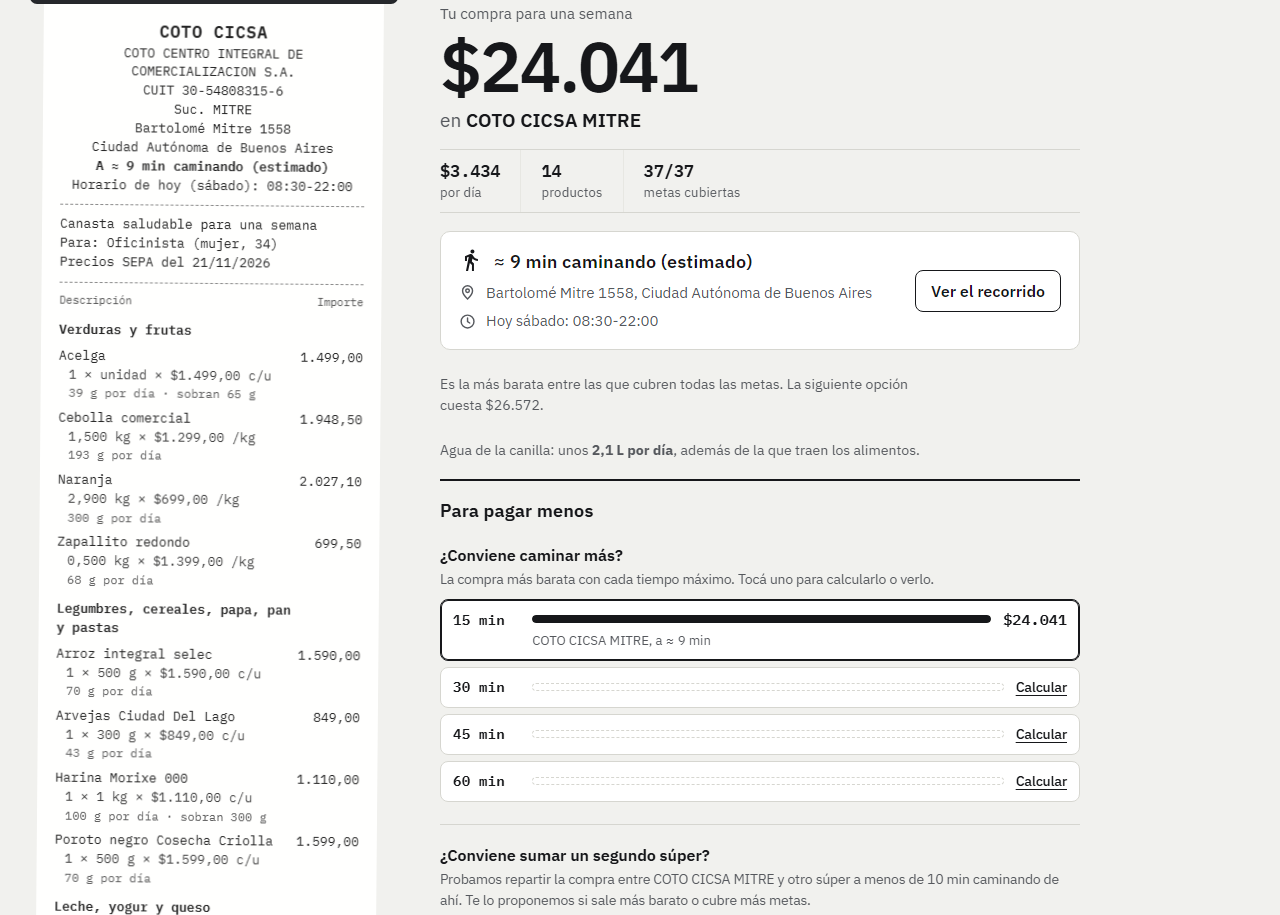
\includegraphics[width=0.66\linewidth]{figuras/resultado.png}
\caption{La respuesta de la página para el caso base: total, sucursal, minutos a
pie, metas cubiertas y el ticket. La página lo resolvió con el motor del navegador y
llegó a \pesos{24.041}; el de Python, a \pesos{24.031}. La diferencia (0,04\,\%) está
dentro del gap del 1\,\% (Sección~\ref{sec:resolucion}).}
\label{fig:resultado}
\end{figure}

\subsection{Aumentar de peso}
\label{sec:aumentar}

El docente nos pidió que la página distinguiera \textbf{aumentar de peso} de
\textbf{ganar masa muscular}. Ninguno de los dos objetivos agrega restricciones:
cambian dos parámetros de la persona. La energía $E_i$ (y con ella la banda de la
restricción \eqref{r:energia}) pasa del gasto diario a $\text{gasto} + 500$\,kcal
para aumentar, que es subir de a poco, como recomienda el NHS a los adultos con bajo
peso \cite{nhs}, o a $\text{gasto} \times 1{,}10$ para masa muscular. El mínimo de
proteína pasa de 0,8 a 1,6\,g por kg para ganar músculo, dentro del rango que
recomienda la ISSN para quien entrena \cite{issn}, y a 1,2\,g por kg para aumentar
de peso: una proteína moderada, porque en ese caso lo que se busca es energía y no
músculo. La Tabla~\ref{tab:aumentar} compara los tres objetivos para la misma
persona.

\begin{table}[H]
\centering\small
\caption{Estudiante de 20 años, 52\,kg y 1,75\,m (IMC 17), con actividad liviana.
Microcentro, hasta 15 minutos a pie; las tres compras son en Coto y cumplen las 37
metas.}
\label{tab:aumentar}
\begin{tabular}{lrrrr}
\toprule
\textbf{Objetivo} & \textbf{Energía} & \textbf{Proteína mínima} & \textbf{Semana} & \textbf{Diferencia} \\
\midrule
Mantener el peso    & 2.290\,kcal & 0,8\,g/kg (42\,g) & \pesos{23.719} & — \\
Ganar masa muscular & 2.520\,kcal & 1,6\,g/kg (83\,g) & \pesos{24.129} & $+1{,}7\,\%$ \\
Aumentar de peso    & 2.790\,kcal & 1,2\,g/kg (62\,g) & \pesos{24.848} & $+4{,}8\,\%$ \\
\bottomrule
\end{tabular}
\end{table}

Comer 500\,kcal más por día cuesta apenas \pesos{1.129} más por semana. Es del mismo
orden de lo que anticipa el precio sombra de la energía
(Sección~\ref{sec:sensibilidad}): la energía es fácil de conseguir, y lo que
encarece una canasta son otras metas. Con otro perfil, una mujer de 22 años con IMC
16,9, el resultado es parecido: pasa de 1.810 a 2.310\,kcal por día y paga
\pesos{568} más por semana (2,4\,\%). El objetivo se respeta aunque no sea
recomendable: el mismo estudiante con 80\,kg (IMC 26,1, sobrepeso según la OMS
\cite{oms-imc}) recibe 3.440\,kcal y el aviso \cita{Con un IMC de sobrepeso no se
recomienda aumentar de peso; consultá a un profesional}.

\subsection{Metas que no se pueden cumplir}

\begin{table}[H]
\centering\small
\caption{Casos donde ninguna sucursal cubre todo. El modelo devuelve la mejor compra
posible y dice qué falta.}
\label{tab:imposibles}
\renewcommand{\arraystretch}{1.2}
\begin{tabularx}{\linewidth}{@{}p{4.6cm}rrX@{}}
\toprule
\textbf{Hogar y lugar} & \textbf{Semana} & \textbf{Metas} & \textbf{Qué pasa} \\
\midrule
Celíaca, vegana y alérgica a maní, frutos secos, soja y sésamo; Microcentro & \pesos{36.706} & 34/35 & La regla de lácteos (3 porciones por día, de leche o de bebidas vegetales) no tiene \textbf{ningún producto apto} que cuente: sale del modelo con déficit del 100\,\%. Todo lo demás se cumple. \\
Celíaca alérgica a leche, huevo, soja, maní y frutos secos; solo alimentos listos; Córdoba & \pesos{331.689} & 35/37 & El calcio llega al 74\,\% y los lácteos al 67\,\%. Ninguna de las 10 sucursales cumple todo. \\
Oficinista en la meseta de Río Negro & — & — & No hay supermercados con precios en SEPA a menos de 25\,km: \textbf{no hay datos} para plantear el problema. \\
\bottomrule
\end{tabularx}
\end{table}

El segundo caso es el que mejor muestra cómo funciona el criterio lexicográfico. La
sucursal más barata de Córdoba arma la canasta por \pesos{127.041}, también con 2
metas sin cumplir pero con déficits más grandes. La elegida cuesta \textbf{2,6 veces
más} porque se acerca más a las metas. Es lo que le pedimos al modelo, nunca cambiar
nutrición por plata, y también su lado discutible: una mejora chica en el calcio vale
cualquier precio. El redondeo de $\Phi$ al 1\,\% suaviza este efecto pero no lo
elimina (lo retomamos en la Sección~\ref{sec:conclusiones}).

Los gráficos de bala de la página (Figura~\ref{fig:balas}) muestran el resultado de
la etapa~1 meta por meta: la franja es el rango $[L_{ik}, U_{ik}]$, el punto es
$v_{ik}$, y lo que no se cumple aparece primero.

\begin{figure}[H]
\centering
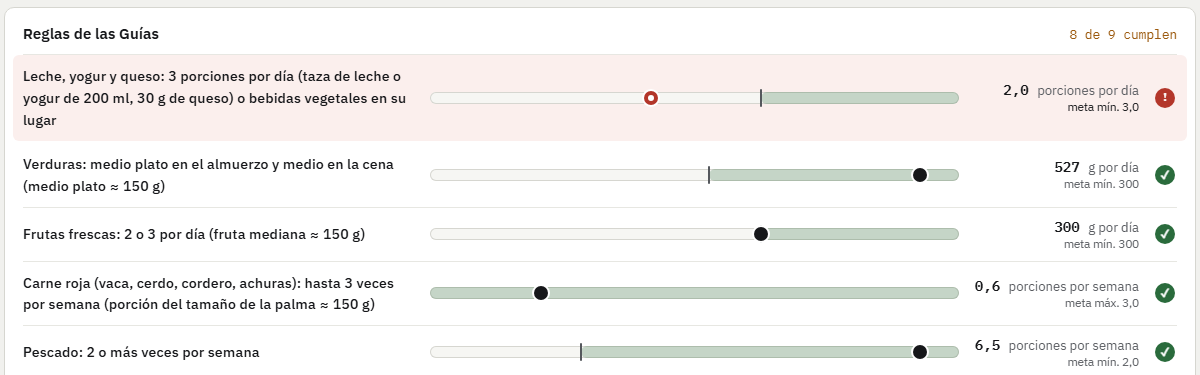
\includegraphics[width=0.82\linewidth]{figuras/balas.png}
\caption{Reglas de las Guías para la persona celíaca con alergias en Córdoba (hogar
con la nena escolar, hasta 30 minutos). La de lácteos llega a 2 de 3 porciones
($\Ddef = 1/3$); las demás quedan dentro de su rango.}
\label{fig:balas}
\end{figure}

\subsection{¿Conviene caminar más?}

Tomamos un hogar de dos personas (una adulta y una nena de 8 años) en el centro de
Córdoba. Al ampliar el tiempo de caminata entran sucursales nuevas (a 45 minutos
entra un Jumbo y sale un Express, por el tope de diez), y la mejor compra baja o se
mantiene:

\begin{table}[H]
\centering\small
\caption{El costo de la misma canasta según cuánto se camina.}
\label{tab:escalera}
\begin{tabular}{rlrrr}
\toprule
\textbf{Hasta} & \textbf{Sucursal elegida} & \textbf{A pie} & \textbf{Semana} & \textbf{Ahorro} \\
\midrule
15 min & Express San Martín      &  2 min & \pesos{56.256} & — \\
30 min & La Anónima Jacinto Ríos & 20 min & \pesos{53.060} & 5,7\,\% \\
45 min & (la misma)              & 20 min & \pesos{53.060} & 5,7\,\% \\
60 min & HiperChangomás Córdoba Este & 57 min & \pesos{42.140} & 25,1\,\% \\
\bottomrule
\end{tabular}
\end{table}

A 15 minutos hay una sucursal más barata (Vea, \pesos{51.930}), pero no cumple 2
metas, así que no se elige. Caminando hasta una hora se ahorra una cuarta parte
respecto de los 15 minutos. Si vale la pena caminar una hora es una decisión de cada
persona, y por eso la página muestra todas las opciones en lugar de decidir sola.

\subsection{¿Conviene un segundo supermercado?}

\begin{itemize}
  \item \textbf{Oficinista en el Microcentro.} Sumar un Express a menos de 10 minutos
        de Coto ahorra \pesos{2.289} (9,5\,\%) con las mismas 37 metas. Supera el
        umbral (3\,\% y \pesos{1.000}), así que la página lo propone.
  \item \textbf{Celíaca con alergias y nena escolar en Córdoba, hasta 30 minutos.} La
        sucursal elegida resuelve el hogar por \pesos{288.518} con 73 de 74 metas.
        Repartiendo con un Express vecino se ahorran \pesos{179.490} (62\,\%) con las
        mismas metas: la primera sucursal se queda con lo que solo ella tiene apto, y
        el resto se compra donde es más barato.
\end{itemize}

\subsection{Promociones}

En el caso base, aplicar o no las promociones \textbf{no cambia la sucursal elegida
ni su total}: ninguna promoción de Coto abarataba esta canasta. Lo que sí cambia es
el orden de las demás: las sucursales de DIA bajan de \pesos{30.617} a \pesos{28.897}
($-5{,}6\,\%$), sin llegar a Coto. Las promociones entran al modelo como una rebaja
con condiciones (Tabla~\ref{tab:promos}), y el ticket muestra el precio de lista, el
descuento y por qué no se aplicó cada una de las que quedaron afuera.

% ============================================================================
\section{Análisis de sensibilidad}
\label{sec:sensibilidad}

Como el modelo tiene variables enteras, estudiamos la sensibilidad de dos maneras:
con la \textbf{relajación lineal} de la etapa~2, que sí tiene precios sombra
\cite{clase-sens}, y con \textbf{barridos}, es decir, volviendo a resolver el modelo
entero cambiando un parámetro por vez. Los barridos ya aparecieron en la
Sección~\ref{sec:casos}: el tiempo de caminata (Tabla~\ref{tab:escalera}), el
período, las promociones y la segunda sucursal.

\paragraph{Qué metas cuestan.} En la relajación del caso base (Oficinista, Coto),
26 de las 36 metas con desvío (todas menos la energía) tienen holgura: aunque las
sacáramos, la compra no bajaría. Las 10 críticas son todas mínimos, y su precio
sombra dice cuánto encarece la semana pedir un 1\,\% más de cada una:

\begin{table}[H]
\centering\small
\caption{Metas críticas de la relajación del caso base, de la más cara a la más
barata. La energía (restricción dura) cuesta \pesos{53} por semana por cada 1\,\%.}
\label{tab:sombra}
\begin{tabular}{lrr}
\toprule
\textbf{Meta crítica} & \textbf{Mínimo} & \textbf{Un 1\,\% más cuesta} \\
\midrule
Calcio                      & 1.000\,mg        & \pesos{38,31} por semana \\
Lácteos (Guías)             & 3 porciones/día  & \pesos{22,56} \\
Verduras (Guías)            & 300\,g/día       & \pesos{21,59} \\
Vitamina B6                 & 1,3\,mg          & \pesos{15,11} \\
Pescado (Guías)             & 2 porciones/semana & \pesos{9,98} \\
Frutas (Guías)              & 300\,g/día       & \pesos{9,36} \\
Vitaminas E, K y A; frutos secos & varios     & \pesos{0,51} a \pesos{2,37} \\
\bottomrule
\end{tabular}
\end{table}

Sacamos dos conclusiones. La primera es que ningún máximo es crítico: con esta
oferta, los topes de sodio, grasas saturadas o carne roja nunca limitan, así que lo
difícil es \emph{llegar} a las metas, no pasarse. La segunda es que la meta más cara
es el calcio, junto con la regla de lácteos. Es justo el par que no se puede cumplir
en Córdoba cuando las alergias sacan los lácteos (Tabla~\ref{tab:imposibles}): el
precio sombra anticipa dónde va a fallar el modelo cuando la oferta se achica.

\paragraph{Lo que cuestan los envases enteros.} La relajación del caso base cuesta
\pesos{16.759} por semana y la compra entera, \pesos{24.031}: un 43\,\% más. Como la
relajación es lineal en el período $D$, para un mes costaría
$16.759 \times 30/7 = \pesos{71.825}$, y la compra entera cuesta \pesos{76.209},
apenas un 6\,\% más. En una semana sobra buena parte de cada paquete; en un mes se
aprovecha. Eso explica por qué el costo por día baja un 26\,\% cuando se compra para
un mes (Tabla~\ref{tab:cumplen}).

% ============================================================================
\section{Librerías utilizadas}
\label{sec:librerias}

\begin{table}[H]
\centering\small
\caption{Librerías y servicios, y para qué usamos cada uno.}
\label{tab:librerias}
\renewcommand{\arraystretch}{1.2}
\begin{tabularx}{\linewidth}{@{}lp{1.6cm}X@{}}
\toprule
\textbf{Librería} & \textbf{Versión} & \textbf{Uso} \\
\midrule
HiGHS \cite{highs}                 & (en SciPy) & El solver de las dos etapas: símplex o punto interior para los programas lineales, y \emph{branch and bound} para los enteros. \\
SciPy (\texttt{optimize}) \cite{scipy} & 1.15   & Para usar HiGHS desde Python: \texttt{linprog} (etapa~1 y relajaciones) y \texttt{milp} (etapa~2, con enteros, gap y límite de tiempo). \\
SciPy (\texttt{sparse}) \cite{scipy}   & 1.15   & Matrices dispersas: la matriz de restricciones tiene miles de columnas y casi todo ceros, con bloques por persona. \\
\texttt{highs} (npm) \cite{highsjs}   & 1.15.4 & HiGHS compilado a WebAssembly: el mismo modelo se resuelve en el navegador, sin servidor. \\
NumPy \cite{numpy}, pandas \cite{pandas}, PyArrow \cite{arrow} & 2.2, 2.2, 21 & Armar los coeficientes $a_{kp}$, los precios y la aptitud a partir de la base (tablas en Parquet). \\
scikit-learn \cite{sklearn}        & 1.6    & Construcción de la base: similitud de nombres (TF-IDF) y clasificación de productos en categorías de góndola. \\
Leaflet \cite{leaflet} y OpenRouteService \cite{ors} & 1.9.4 & Mapa de la página y tiempos de caminata reales. No intervienen en la optimización. \\
\bottomrule
\end{tabularx}
\end{table}

% ============================================================================
\section{Conclusiones}
\label{sec:conclusiones}

\begin{itemize}
  \item \textbf{El problema de la dieta sigue sirviendo si se lo completa.} Con
        variedad, envases enteros y metas con máximo, el óptimo deja de ser ``harina
        y repollo'' y pasa a ser una compra que alguien haría de verdad: 14
        productos, de cinco grupos de alimentos, por \pesos{24.031} la semana.
  \item \textbf{Con el modelo lexicográfico no tuvimos que ponerle precio a la
        salud.} Las dos etapas responden, en orden, ``¿qué es lo mejor que se puede
        comer acá?'' y ``¿cuánto es lo menos que cuesta?''. Una meta imposible no
        vuelve infactible al modelo: se mide y se informa. La única restricción dura
        es la energía.
  \item \textbf{Dónde comprar pesa tanto como qué comprar.} La misma canasta puede
        costar hasta 3 veces más según la sucursal, caminar más puede ahorrar un
        25\,\% y repartir la compra, más de la mitad en hogares con muchas
        restricciones.
\end{itemize}

\needspace{6\baselineskip}
\paragraph{Limitaciones.}
\begin{itemize}
  \item El orden lexicográfico puede pagar mucho por una mejora nutricional chica,
        como en el caso de Córdoba. Una mejora natural sería el método de la
        $\varepsilon$-restricción \cite{chankong}: resolver la etapa~2 con
        $\Phi \leq \Phi^\ast + \varepsilon$ para varios valores de $\varepsilon$ y
        mostrar la curva entre costo y cumplimiento, para que la persona elija.
  \item Quedarnos solo con las subcategorías de la relajación en la etapa~2 es una
        heurística: no garantiza el óptimo entero global, aunque en la práctica la
        diferencia es chica.
  \item La canasta es por día promedio: no arma menús ni comidas, y las reglas
        semanales de las Guías se cumplen en promedio.
  \item Los nutrientes de los productos sin rótulo salen de alimentos genéricos, y
        los precios son los que se publican en SEPA, que no tienen en cuenta si hay
        faltantes de stock.
\end{itemize}

% ============================================================================
\begin{thebibliography}{99}

\bibitem{stigler} Stigler, G. J. (1945). \emph{The Cost of Subsistence}. Journal of
  Farm Economics, 27(2), 303--314.

\bibitem{dantzig} Dantzig, G. B. (1990). \emph{The Diet Problem}. Interfaces, 20(4),
  43--47. \url{https://doi.org/10.1287/inte.20.4.43}

\bibitem{garille} Garille, S. G. y Gass, S. I. (2001). \emph{Stigler's Diet Problem
  Revisited}. Operations Research, 49(1), 1--13.

\bibitem{highs} Huangfu, Q. y Hall, J. A. J. (2018). \emph{Parallelizing the dual
  revised simplex method}. Mathematical Programming Computation, 10(1), 119--142.
  Solver HiGHS: \url{https://highs.dev}

\bibitem{clase-formulacion} Cátedra de Optimización, UCA (2025). \emph{Clase 02:
  Formulación general}. Modelos de formulación de productos: el problema de la dieta
  (Green Nutrition).

\bibitem{clase-sens} Cátedra de Optimización, UCA (2025). \emph{Clase 03:
  Sensibilidad}. Análisis post-óptimo: holguras, precio sombra, costo reducido y
  rango de variación.

\bibitem{clase-metas} Cátedra de Optimización, UCA (2025). \emph{Clase 05:
  Programación lineal por objetivos o metas}. Desvíos por defecto y por exceso,
  metas ponderadas y metas lexicográficas.

\bibitem{clase-mip} Cátedra de Optimización, UCA (2025). \emph{Clase 06:
  Programación lineal entera y binaria}. Ramificación y acotamiento, variables
  binarias y operadores lógicos.

\bibitem{hillier} Hillier, F. S. y Lieberman, G. J. (2015). \emph{Introducción a la
  Investigación de Operaciones} (9.\textsuperscript{a} ed.). México: McGraw-Hill.
  Programación por metas.

\bibitem{sepa} Secretaría de Comercio Interior. \emph{Precios Claros — Base SEPA}.
  Datos abiertos, archivo del 21/11/2026.
  \url{https://datos.produccion.gob.ar/dataset/sepa-precios}

\bibitem{guias} Ministerio de Salud de la Nación (2016). \emph{Guías Alimentarias para
  la Población Argentina}. Documento técnico metodológico.

\bibitem{fao} FAO/OMS/UNU (2004). \emph{Human Energy Requirements}. Serie de Informes
  Técnicos sobre Alimentación y Nutrición 1.

\bibitem{dri} Institute of Medicine (1997--2005). \emph{Dietary Reference Intakes}.
  National Academies Press.

\bibitem{oms-azucares} Organización Mundial de la Salud (2015). \emph{Guideline: Sugars
  intake for adults and children}. Ginebra: OMS.

\bibitem{oms-grasas} Organización Mundial de la Salud (2023). \emph{Saturated fatty
  acid and trans-fatty acid intake for adults and children: WHO guideline}. Ginebra:
  OMS.

\bibitem{oms-imc} Organización Mundial de la Salud (2000). \emph{Obesity: preventing
  and managing the global epidemic}. Serie de Informes Técnicos 894. Ginebra: OMS.

\bibitem{nhs} National Health Service del Reino Unido. \emph{Advice for underweight
  adults}. Consejo para adultos con bajo peso, consultado en noviembre de 2026.
  \url{https://www.nhs.uk/live-well/healthy-weight/managing-your-weight/advice-for-underweight-adults/}

\bibitem{issn} Jäger, R. et al. (2017). \emph{International Society of Sports
  Nutrition Position Stand: protein and exercise}. Journal of the International
  Society of Sports Nutrition, 14, 20.

\bibitem{chankong} Chankong, V. y Haimes, Y. Y. (1983). \emph{Multiobjective Decision
  Making: Theory and Methodology}. Nueva York: North-Holland.

\bibitem{off} Open Food Facts. \emph{Base de datos abierta de productos
  alimenticios} (licencia ODbL). Volcado consultado en noviembre de 2026.
  \url{https://world.openfoodfacts.org}

\bibitem{usda} U.S. Department of Agriculture, Agricultural Research Service (2018).
  \emph{FoodData Central: SR Legacy}. \url{https://fdc.nal.usda.gov}

\bibitem{catalogos} Cencosud. Catálogos online de Jumbo, Disco y Vea (rótulos,
  ingredientes y categorías de góndola), consultados en noviembre de 2026.
  \url{https://www.jumbo.com.ar}, \url{https://www.disco.com.ar},
  \url{https://www.vea.com.ar}

\bibitem{ors} HeiGIT (Heidelberg Institute for Geoinformation Technology).
  \emph{openrouteservice}, perfil peatonal \texttt{foot-walking}.
  \url{https://openrouteservice.org}

\bibitem{osm} Colaboradores de OpenStreetMap. \emph{OpenStreetMap} (licencia ODbL).
  \url{https://www.openstreetmap.org}

\bibitem{scipy} Virtanen, P. et al. (2020). \emph{SciPy 1.0: fundamental algorithms
  for scientific computing in Python}. Nature Methods, 17, 261--272.

\bibitem{numpy} Harris, C. R. et al. (2020). \emph{Array programming with NumPy}.
  Nature, 585, 357--362.

\bibitem{pandas} McKinney, W. (2010). \emph{Data structures for statistical computing
  in Python}. Proceedings of the 9th Python in Science Conference, 56--61.

\bibitem{arrow} Apache Software Foundation. \emph{Apache Arrow} (PyArrow 21).
  \url{https://arrow.apache.org}

\bibitem{sklearn} Pedregosa, F. et al. (2011). \emph{Scikit-learn: machine learning
  in Python}. Journal of Machine Learning Research, 12, 2825--2830.

\bibitem{highsjs} Lojkine, O. \emph{highs-js}: HiGHS compilado a WebAssembly, paquete
  npm \texttt{highs} 1.15.4. \url{https://github.com/lovasoa/highs-js}

\bibitem{leaflet} Agafonkin, V. \emph{Leaflet} 1.9.4: librería de mapas interactivos.
  \url{https://leafletjs.com}

\bibitem{pagina} Martínez Folica, N. y Naón, P. (2026). \emph{Canasta saludable}:
  página publicada del trabajo, con la base del día.
  \url{https://nazarenofolica.github.io/Optimizacion_TPS/}

\end{thebibliography}

% ============================================================================
\section*{Anexo — Verificación}
\addcontentsline{toc}{section}{Anexo — Verificación}

\begin{itemize}
  \item Escribimos 254 tests de Python que cubren la construcción de la base, los
        requerimientos, el modelo (incluido el ejemplo de la
        Sección~\ref{sec:juguete}), las promociones, las rutas y el servidor local.
        Se corren solos en cada cambio, con GitHub Actions.
  \item Un test de paridad resuelve los mismos casos con el motor de Python y con el
        de la página (HiGHS en WebAssembly, en Chrome) y compara la compra, las metas
        y los avisos: los 4 casos coinciden dentro de la tolerancia.
  \item El código, los datos y la página están en el repositorio del trabajo
        (carpeta \texttt{TPF/}), y la página se puede usar sin instalar nada
        \cite{pagina}.
\end{itemize}

\end{document}
